\chapter[Raíces de funciones de una variable]{Interpolación y
  aproximación de funciones%
  \footnote{\licenseInfo}}
 \label{cha:Interpolacion-aproximacion}

 El problema de la interpolación surge cuando se intenta construir una
 función (a la que suele llamarse función interpolante) de la que
 solamente conocemos sus valores en una serie de puntos (que suelen
 llamarse nodos de interpolación).  Este tipo de problemas surge, por
 ejemplo, si disponemos de un cierto número de datos puntos obtenidos
 por muestreo o a partir de un experimento y pretendemos construir una
 función que los ajuste, o bien si pretendemos aumentar el tamaño de
 una fotografía, rellenando la imagen inicial con datos que son
 <<inventados>>.

 Un problema estrechamente ligado con el de la interpolación es la
 aproximación de una función complicada por una más simple y por tanto
 más fácil de manejar (derivar, integrar, etc). Por ejemplo, los
 métodos usuales para la aproximación de la integral de una función en
 un intervalo se basan en sustituirla por una función polinómica.  En
 lo que sigue, supondremos que la función interpolante es un polinomio
 (aunque existen otras posibilidades: interpolación por funciones
 racionales, trigonométricas, exponenciales, etc.), puesto que son las
 funciones más sencillas de manejar y constituyen la base de los
 métodos numéricos que estudiaremos en los próximos capítulos.

 \section{Interpolación de Lagrange}
 \label{sec:interp-de-lagrange}

 Consideremos conjunto de datos definido por un soporte de $n+1$ nodos
 distintos, $S=\{x_0,x_1,\dots,x_n\}\subset \Rset$, junto a $n+1$
 puntos $y_i \in \Rset$:
 \newcolumntype{g}{>{\columncolor{lightgray}}r}
 \begin{equation}
   \begin{array}{grrrcr}
     \toprule
     x & x_0 & x_1 & x_2 & \dots & x_n
     \\ %\midrule
     y & y_0 & y_1 & y_2 & \dots & y_n
     \\
     \bottomrule
   \end{array}
   \label{eq:tabla-datos-lagrange}
 \end{equation}
 y denotemos por $\Pol_n[x]$ al conjunto de los polinomios de grado
 menor o igual a $n$ en la variable $x$. Planteamos el problema de la
 interpolación de Lagrange como:
 \begin{equation}
   \tag{P$_{IL}$}
   \text{Hallar } p\in\Pol_n[x] \tq p(x_i)=y_i \quad \forall i=0,1,\dots,n.
   \label{eq:problema-interpol-lagrange}
 \end{equation}
 \begin{definition}
   \label{def:interpolador-lagrange}
   Decimos que un polinomio $p$ interpola el conjunto de
   datos~\eqref{eq:tabla-datos-lagrange} si $p$ es solución del
   problema~\eqref{eq:problema-interpol-lagrange}. En el caso en que
   los datos vengan dados por una función, $y_i=f(x_i)$ decimos que $p$
   es el polinomio de interpolación de Lagrange (o interpolador de
   Lagrange) de la función $f$ en los nodos $x_0$, $x_1$, \dots, $x_n$.
 \end{definition} 
 En adelante supondremos $f\in C^0([a,b])$ para cierto intervalo
 $[a,b]\subset\Rset$ que contiene a los nodos de interpolación,
 $x_0,x_1,\dots,x_n \in [a,b]$.  El resto de esta sección se estructura
 de la siguiente forma:
 \begin{enumerate}
 \item Estudio de la existencia y unicidad de solución del
   problema~\eqref{eq:problema-interpol-lagrange}.
 \item Deducción de algoritmos para el cálculo efectivo del polinomio
   de interpolación.
 \item Análisis del error de interpolación, es decir de la diferencia
   $|f(x)-p(x)|$ con $x\in [a,b]$.
 \end{enumerate}

 \subsection{Existencia y unicidad del interpolador de Lagrange}
 \label{sec:exist-y-unic-lagrange}

 \begin{theorem}
   \label{thm:existencia-unicidad-lagrange}
   Dado un soporte de $n+1$ nodos distintos $x_0$, $x_1$,\dots, $x_n
   \in \Rset$ y dados $y_0$, $y_1$,\dots, $y_n\in\Rset$ cualesquiera,
   existe una única solución de~\eqref{eq:problema-interpol-lagrange},
   es decir existe un único polinomio $p\in\Pol_n[x]$ tal que
   $p(x_i)=y_i$ para todo $i=0,1,\dots,n$.
 \end{theorem}
 \begin{proof}~
   \etapa{Etapa a) Equivalencia con un sistema lineal de ecuaciones.}
   Todo polinomio $p\in\Pol_n[x]$, está unívocamente determinado por
   $n+1$ coeficientes, $a_0$, $a_1$, \dots, $a_n\in\Rset$ tales que
   \begin{equation}
     p(x)=a_0 + a_1 x + \cdots + a_n x^n.
   \end{equation}
   A su vez, el polinomio de interpolación se caracteriza por verificar
   $n+1$ ecuaciones,
   $$
   p(x_i)=y_i, \quad i=0,1,\dots,n,
   $$
   que se pueden escribir como el siguiente sistema de $n+1$ ecuaciones
   con $n+1$ incógnitas (cuya matriz cuadrada, $A$, se conoce como
   matriz de Vandermonde):
   \begin{equation}
     \begin{pmatrix}
       1 & x_0& \cdots & x_0^n \\
       1 & x_1& \cdots & x_1^n \\
       \vdots & \vdots & & \vdots \\
       1 & x_n& \cdots & x_n^n 
     \end{pmatrix}
     \begin{pmatrix}
       a_0 \\ a_1 \\ \vdots \\ a_n
     \end{pmatrix}
     =
     \begin{pmatrix}
       y_0 \\ y_1 \\ \vdots \\ y_n
     \end{pmatrix}.
   \end{equation}
   Por tanto la existencia y unicidad del polinomio de interpolación es
   equivalente a la existencia de unos únicos coeficientes
   $(a_0,a_1,...,a_n)$ que solucionan el sistema anterior.

   \etapa{Etapa b) Existencia y unicidad de solución.}  Veremos que
   este sistema tiene una única solución. Para ello, como $A$ es una
   matriz cuadrada, basta ver que $|A|\neq 0$, para lo que es suficiente
   probar que el sistema homogéneo $Au=0$, con $u\in\Rset^{n+1}$, tiene
   como única solución $u=0$.

   Supongamos que $u=(a_0,a_1,\dots,a_n) \in\Rset^{n+1}$ verifica
   $Au=0$. Entonces, el polinomio asociado, $p(x)=a_0 + a_1x + \cdots
   + a_n x^n$, verifica $p(x_i)=0$ para $i=0,1,\dots,n$.  Por lo tanto $p$ es un
   polinomio de grado $n$ con $n+1$ raíces distintas, luego
   $p=0$, es decir $u=(a_0,a_1,\dots,a_n)=0$. 
 \end{proof}

 \begin{remark}
   \label{rk:1}
   En la demostración anterior podríamos haber probado directamente
   que el determinante de la matriz de Vandermonde es distinto de cero,
   pues los puntos $x_0$, $x_1$, \dots, $x_n$ son distintos
   entre sí. Pero se ha optado por realizar la etapa b) debido a que el
   argumento empleado (es decir, en un sistema lineal con matriz
   cuadrada, la unicidad [o sea $Au=0 \Rightarrow u=0$] implica la existencia)
   es generalizable a otras demostraciones de existencia y unicidad que
   aparecerán, por ejemplo, en la siguiente sección.
 \end{remark}

 \subsection{Construcción del polinomio de interpolación de Lagrange}
 \label{sec:construcion--polinomio-lagrange}

 De la demostración del Teorema~\ref{thm:existencia-unicidad-lagrange}
 se puede deducir un primer método para la construcción del
 interpolador de Lagrange: la resolución del sistema lineal con matriz
 de Vandermonde. Sin embargo, este método es costoso, pues se trata de
 una matriz llena (con pocos ceros) y además se puede demostrar que
 esta matriz tiene un mal condicionamiento cuando $n$ crece hacia
 infinito. Estudiaremos dos métodos más adecuados.

 \subsubsection{Fórmula de Lagrange}
 Dado un soporte de $n+1$ puntos distintos, $S=\{x_0,x_1,\dots,x_n\}$,
 existe un único polinomio $L_i\in \Pol_n[x]$, que interpola los
 valores $y_0=0$, \dots, $y_{i-1}=0$, $y_i=1$, $y_{i+1}=0$, \dots,
 $y_n=0$ (debido al Teorema~\ref{thm:existencia-unicidad-lagrange}). Es
 decir, $L_i$ verifica (para cada $x_j$):
 \begin{equation}
   L_i(x_j)= \delta_{ij} = 
   \left\{\begin{array}{l}
       1 \text{ si } i=j, \\\noalign{\medskip} 0 \text{ si } i\neq j
     \end{array}\right. \quad \text{(función delta de Kronecker).}
 \end{equation}
 En concreto, es fácil comprobar que el polinomio $L_i(x)$ viene dado
 por el siguiente polinomio (de orden exactamente igual a $n$):
 \begin{equation}
   L_i(x)=
   \begin{array}{c@{}c@{}c@{}c@{}c@{}c@{}c}
     (x-x_0) & \cdots & (x-x_{i-1}) & \cdot & (x-x_{i+1}) & \cdots &
     (x-x_n)
     \\ \hline
     (x_i-x_0) & \cdots & (x_i-x_{i-1}) & \cdot & (x_i-x_{i+1}) & \cdots &
     (x_i-x_n)
   \end{array}
   % \frac{x-x_0}{x_i-x_0}\cdots
   % \frac{x-x_{i-1}}{x_i-x_{i-1}}\cdot
   % \frac{x-x_{i+1}}{x_i-x_{i+1}}\cdots
   % \frac{x-x_n}{x_i-x_n}.
 \end{equation}
 El conjunto de los polinomios $\{ L_0, L_1,\dots, L_n \}$ se llama
 base de Lagrange asociada al soporte $S=\{x_0,x_1,\dots,x_n\}$. 

 Así, dado un conjunto de valores $\{y_0,y_1,\dots,y_n\}$, el polinomio
 que los interpola en el soporte $S$ viene dado por la siguiente
 combinación lineal:
 \begin{equation}
   p(x)= y_0L_0(x) + y_1 L_1(x) + \cdots + y_n L_n(x),
 \end{equation}
 pues, por construcción de los polinomios $L_i$, el polinomio anterior
 es solución de~(\ref{eq:problema-interpol-lagrange}).

 \begin{example}
   \label{sec:formula-de-lagrange}
   Calculemos el polinomio de interpolación de Lagrange asociado a
   los puntos:
   \begin{align*}
     (x_0, y_0)&=(-1,0), &\quad (x_2, y_2)&=(1,2),\\ 
     (x_1, y_1)&=(0,2),   &\quad (x_3, y_3)&=(2,6).
   \end{align*}
   La base de Lagrange asociada al soporte
   $S=\{x_0,x_1,x_2,x_3\}=\{-1,0,1,2\}$ es:
   \begin{small}
     \begin{align*}
       L_0(x) & =
       \frac{(x-x_1)(x-x_2)(x-x_3)}{(x_0-x_1)(x_0-x_2)(x_0-x_3)} =
       \frac{(x-0)(x-1)(x-2)}{(-1-0)(-1-1)(-1-2)} =
       -{{\left(x-2\right)\,\left(x-1\right)\,x}\over{6}}, \\
       \noalign{\medskip} L_1(x) & =
       \frac{(x-x_0)(x-x_2)(x-x_3)}{(x_1-x_0)(x_1-x_2)(x_1-x_3)} =
       \frac{(x+1)(x-1)(x-2)}{(0+1)(0-1)(0-2)} =
       {{\left(x-2\right)\,\left(x-1\right)\,\left(x+1\right)}\over{2}},
       \\ \noalign{\medskip} L_2(x) & =
       \frac{(x-x_0)(x-x_1)(x-x_3)}{(x_2-x_0)(x_2-x_1)(x_2-x_3)} =
       \frac{(x+1)(x-0)(x-2)}{(1+1)(1-0)(1-2)} =
       -{{\left(x-2\right)\,x\,\left(x+1\right)}\over{2}}, \\
       \noalign{\medskip} L_3(x) & =
       \frac{(x-x_0)(x-x_1)(x-x_2)}{(x_3-x_0)(x_3-x_1)(x_3-x_2)} =
       \frac{(x+1)(x-0)(x-1)}{(2+1)(2-0)(2-1)} =
       {{\left(x-1\right)\,x\,\left(x+1\right)}\over{6}}.
     \end{align*}
   \end{small} 
   Así tenemos el polinomio de interpolación para los valores
   $\{y_0,y_1,y_2,y_3\}=\{0,2,2,6\}$:
   \begin{align*}
     p(x)&= \sum_{i=0}^3 y_iL_i(x) 
     = 0\cdot L_0(x) + 2\cdot L_1(x)+ 2\cdot L_2(x)+6\cdot L_3(x)
     \\ &=(x-1)x(x+1)-(x-2)x(x+1)+(x-2)(x-1)(x+1)
     =x^3-x^2+2.
   \end{align*}
   Podemos comprobar que no hubo errores, pues efectivamente $p(x)$ es
   un polinomio que interpola los valores
   $(x_i,y_i)$ (el único de $\Pol_3[x]$ que lo hace):
   \begin{align*}
     p(x_0)&=p(-1)=(-1)^3-(-1)^2+2=0=y_0, & p(x_2)&=1^3-1^2+2 = 2=y_2, \\
     p(x_1)&=p(0) = 2=y_1, & p(x_3)&=2^3-2^2+2 = 6=y_3.
   \end{align*}
 \end{example}

 \begin{remark}
   Una ventaja de la fórmula de Lagrange es que, fijado un soporte $S$
   y una vez calculados los polinomios $\{L_0,L_1,\dots, L_n\}$ que
   forman a la base de Lagrange asociada, es muy sencillo calcular los
   polinomios que interpolan tantos conjuntos de valores,
   $\{y_0,y_1,\dots,y_n\}$ como deseemos. 

   Sin embargo, su inconveniente es que si deseamos añadir un punto más
   al soporte (y por tanto realizar la interpolación con un polinomio
   de un grado mayor) es necesario volver a calcular toda la base de
   polinomios de Lagrange.
 \end{remark}

 \subsubsection{Fórmula de Newton}
 \label{sec:formula-de-newton}
 A continuación, dado el soporte $S=\{x_0,x_1,\dots,x_n\}$ de $n+1$ puntos
 distintos y dados $n+1$ valores $\{y_0,y_1,\dots,y_n\}$, sea
 $p_n$ el (único) polinomio $p_n \in \Pol_n[x]$, que
 interpola los valores $\{y_i\}_{i=0}^n$, es decir
 \begin{equation}
   p_n(x_i)=y_i, \quad \forall i=0,...,n.
   \label{eq:interpol.1}
 \end{equation}
 Expresaremos este polinomio de la siguiente forma:
 \begin{align}
   \notag
   p_n(x)&=a_0 + a_1 (x-x_0) + a_2(x-x_0)(x-x_1) + \cdots 
   + a_n(x-x_0)(x-x_1)\cdots(x-x_{n-1}) \\
   &=\sum_{k=0}^n a_k \prod_{i=0}^{k-1}(x-x_i),
   \label{eq:pol.newton.dif-div}
 \end{align}
 donde $a_0$, $a_1$, \dots, $a_n\in\Rset$ son coeficientes que se
 pueden ajustar para que se verifiquen las
 ecuaciones~(\ref{eq:interpol.1}):
 \begin{align*}
   p_n(x_0)&=y_0 \Rightarrow a_0=y_0.\\
   p_n(x_1)&=y_1 \Rightarrow a_0+a_1(x_1-x_0)=y_1 
   \Rightarrow a_1=\frac{y_1-y_0}{x_1-x_0}.\\
   p_n(x_2)&=y_2 \Rightarrow a_0+a_1(x_2-x_0)+a_2(x_2-x_0)(x_2-x_1)=y_2 
   \Rightarrow a_2=\cdots\\
   &\vdots
 \end{align*}
 Estos coeficientes se pueden calcular mediante una regla de
 recurrencia sencilla, conocida como fórmula de las diferencias dividas
 de Newton, que veremos a continuación. Históricamente se ha utilizado
 la siguiente notación (en la que se asume que los datos vienen dados
 por cierta función, $y_k=f(x_k)$, y se expresa el hecho de que cada
 $a_k$ depende solamente de los valores de $f$ en
 $\{x_0,x_1,\dots,x_k\}$):
 % De forma más compacta, podemos escribir:
 % \begin{equation}
 %   p_n(x)=\sum_{k=0}^n a_k \prod_{i=0}^{k-1}(x-x_i).
 %   \label{eq:interpol.2}
 % \end{equation}
 \begin{definition}
   Dada una función $f$ de la cual se conocen los valores $y_0=f(x_0)$,
   $y_1=f(x_1)$, \dots, $y_n=f(x_n)$, 
   a cada uno de los coeficientes, $a_k$, del polinomio $p_n(x)$
   anterior se le llama \resaltar{diferencia
     dividida} (de orden $k$) de $f$ en los nodos $x_0$, $x_1$, \dots
   $x_n$. La diferencia dividida de orden $k$ se denota como
   $$
   a_k = f[x_0,x_1,\dots,x_k].
   $$
 \end{definition}

 El siguiente lema expresa las propiedad más importante de las
 diferencias divididas%
 \footnote{El lector interesado en estudiar más a fondo las
   diferencias divididas  puede consultar por ejemplo la
   siguiente referencia Bibliográfica: Kincaid, D., Cheney, W.,
   Análisis Numérico. \textit{Las matemáticas del cálculo
     científico}. Addison-Wesley-Iberoamericana 1994.}.
 % \begin{lemma}
 %   \label{lem:interpol1}
 %   El polinomio de interpolación de los datos $y_i=f(x_i)$ se puede
 %   escribir como
 %   $$
 %   p(x) = a_0 + a_1x + a_2x^2 + \cdots a_nx^n,
 %   $$
 %   donde cada $a_k=f[x_0,...,x_k]$.
 % \end{lemma}
 % \begin{proof}
 %   Consideremos el polinomio de interpolación, para los valores
 %   $y_i=f(x_i)$, $i=0,...,n$, que hemos expresado de la
 %   forma~(\ref{eq:pol.newton.dif-div}). Por definición, cada
 %   $a_k=f[x_0,...,x_k]$.

 %   Si observamos último sumando de tenemos que
 %   $$
 %   (x-x_0)(x-x_1)\cdots (x-x_{n-1}) = x^n + \text{términos de grado
 %   menor que $n$},
 %   $$
 %   por lo tanto $a_n=f[x_0,...,x_n]$ es el coeficiente de $x^n$ en el
 %   polinomio de interpolación.

 %   Consideremos ahora el polinomio resultante de truncar el último sumando:
 %   \begin{align*}
 %     p_{n-1}(x)= \sum_{k=0}^{n-1} a_k \prod_{i=0}^{k-1}(x-x_i).
 %   \end{align*}
 %   Es fácil ver que $p_{n-1}$ es el único polinomio de grado $n-1$ que
 %   interpola los valores $(x_i,y_i)$ para $i=0,...,n-1$. En concreto,
 %   %   \begin{equation*}
 %     $  p_{n-1}(x)  =p_n(x)-a_n \prod_{i=0}^{n-1}(x-x_i),$
 %   %   \end{equation*}
 %   luego $p_{n-1}(x_i)=y_i$ para $i=0,\dots,n-1$, es decir $p_{n-1}$
 %   es el (único) polinomio de interpolación de estos datos.

 %   Si miramos el último sumando de $p_{n-1}(x)$, tenemos 
 %   $$
 %   (x-x_0)(x-x_1)\cdots (x-x_{n-2}) = x^{n-1} + \text{términos de grado
 %   menor que $n-1$},
 %   $$
 % %   
 % \end{proof}
 % 

 \begin{lemma}
   \label{lem:1}
   Las formulas divididas satisfacen la siguiente relación recursiva:
   \begin{equation}
     \begin{aligned}
       f[x_i]&=y_i, \quad i=0,...n,
       \\
       f[x_0,x_1,\dots,x_n]&=
       \frac{f[x_1,x_2,\dots,x_n]-f[x_0,x_1,\dots,x_{n-1}]}{x_n - x_0}.
     \end{aligned}
     \label{eq:interpol.dif-div.recursiva}
   \end{equation}
 \end{lemma}
 En~(\ref{eq:interpol.dif-div.recursiva}), los puntos
 $x_0,...,x_n$ deben interpretarse como variables, en un sentido amplio
 (pues de hecho $\{x_k\}_{k=0}^n$ son puntos genéricos, con $n$
 cualquiera, y podrían volver a enumerarse de cualquier otra forma, por
 ejemplo $\{x_k\}_{k=i}^{i+j}$). Por lo tanto, son ciertas todas las
 ecuaciones del tipo
 \begin{equation*}
   f[x_i,x_{i+1},\dots,x_{i+j}]=
   \frac{f[x_{i+1},\dots,x_{i+j}]-f[x_i,\dots,x_{i+j-1}]}{x_j - x_i}.
 \end{equation*}

 Aunque la demostración del lema anterior es de carácter técnico, la
 incluimos de modo ilustrativo.
 \begin{proof}~ 
   \etapa{Etapa 1.} Sean $p_n\in\Pol_n[x]$ y $p_{n-1}\in
   \Pol_{n-1}[x]$ los polinomios de interpolación de los valores
   $\{x_i,f(x_i)\}_{i=0}^n$ y $\{x_i,f(x_i)\}_{i=0}^{n-1}$,
   respectivamente. Sea $q_{n-1}\in\Pol_{n-1}[x]$ el polinomio de
   interpolación de $\{x_i,f(x_i)\}_{i=1}^{n}$.

   Entonces, se verifica:
   \begin{equation}
     p_n(x)=q_{n-1}(x)+\frac{x-x_n}{x_n-x_0}\left[q_{n-1}(x)-p_{n-1}(x)\right].\label{eq:1}
   \end{equation}
   Esto es debido a que (como es fácil comprobar usando la definición
   de $p_{n-1}$ y $q_{n-1}$) el segundo miembro es un polinomio de
   grado $n$ que interpola los valores $\{x_i,f(x_i)\}_{i=0}^n$. Luego,
   por unicidad del polinomio de interpolación, tiene que conicidir con
   $p_n$. 

   \etapa{Etapa 2.}  Por definición, $a_n=f[x_0,...,x_n]$ es el
   coeficiente del término $ (x-x_0)(x-x_1)\cdots (x-x_{n-1}) $ en la
   expresión~(\ref{eq:pol.newton.dif-div}) del polinomio de
   interpolación. Pero teniendo en cuenta que
   $$
   (x-x_0)(x-x_1)\cdots (x-x_{n-1}) = x^n + \text{términos de grado
     menor que $n$},
   $$
   $a_n=f[x_0,...,x_n]$ coincide con el coeficiente de $x^n$ en el
   polinomio de interpolación. En general, para todo $j<k$, $f[x_j,...,x_{k}]$ es el
   coeficiente del término de mayor grado en el polinomio que
   interpola los valores $\{x_i,f(x_i)\}_{i=j}^{k}$.

   \etapa{Etapa 3.} A continuación, examinamos los coeficientes del
   término de mayor grado, es decir de $x^n$, en el primer y el
   segundo miembro de~(\ref{eq:1}). Estos coeficientes deben ser
   iguales, lo que nos lleva inmediatamente a la fórmula
   recursiva~(\ref{eq:interpol.dif-div.recursiva}) que buscamos (en el
   segundo miembro de~(\ref{eq:1}) sólo influye el término de mayor
   grado de $q_{n-1}(x)-p_{n-1}(x)$).
 \end{proof}

 El lema~\ref{lem:1} nos permite organizar el cálculo de las
 diferencias divididas a través de un procedimiento sencillo
 \begin{center}
   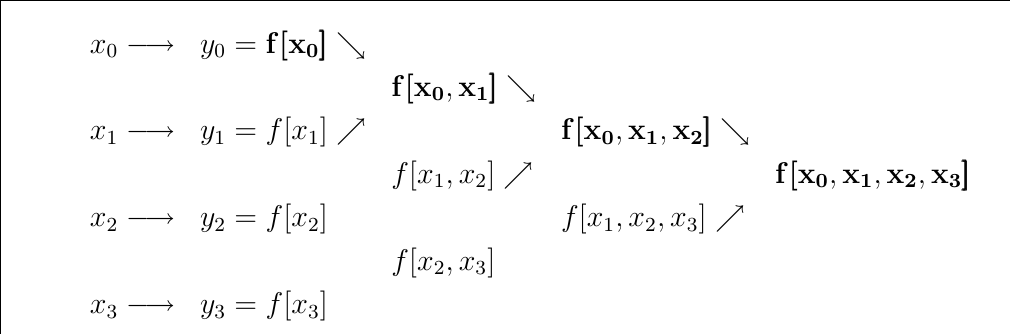
\includegraphics[width=0.9\linewidth]{tema2/diferencias-div}
 \end{center}

 \begin{example}
   Calcular el polinomio de interpolación de Lagrange de $f(x)=2^x$ en
   $S=\{-2,-1,0,1,2\}$. 
 \end{example}

 Una fórmula poco costosa computacionalmente para la evaluación del
 polinomio de interpolación en un punto es la \resaltar{fórmula de
   Ruffini-Horner}: 
 \begin{equation*}
   p_n(r) = a_0 + (r-x_0)(a_1 + (r-x_1)(a_2 + \cdots + (r-x_n)a_n)\cdots)
 \end{equation*}
 En esta fórmula, el número de multiplicaciones se ve reducida
 sustancialmente con con respecto a la
 expresión~(\ref{eq:pol.newton.dif-div}) .
 \begin{example}
   Utilizaremos la interpolación de $f(x)=2^x$ y la fórmula de
   Ruffini-Horner para obtener una aproximación de $\sqrt{2}$.
 \end{example}

 \subsection{Expresión del error}
 \label{sec:error-interpol-lagrange}
 Como antes, consideremos una función $f(x)$ definida en un intervalo
 $[a,b]$ de la que conocemos los valores $y_i=f(x_i)$ en un soporte
 $\{x_0,x_1,\dots,x_n\}$. El siguiente resultado nos ofrece, suponiendo
 regularidad en $f$, una cota del error de interpolación en cada punto
 de $[a,b]$:
 \begin{theorem}
   \label{thm:error-interpol-lagrange}
   Sea $f\in C^{n+1}([a,b])$ y fijemos un soporte de $n+1$ puntos
   distintos, $S=\{x_0,x_1,\dots,x_n\}\subset[a,b]$. Sea
   $p_n\in\Pol_n[x]$ el polinomio de interpolación asociado a los valores
   $y_i=f(x_i)$, $i=0,...,n$. Para cada $x\in[a,b]$, existe $\xi_x\in
   (a,b)$ tal que:
   \begin{equation}
     \label{eq:expresion-error-interpol}
     f(x)-p_n(x)=\frac{f^{n+1)}(\xi_x)}{(n+1)!} (x-x_0)(x-x_1)\dots(x-x_n).
   \end{equation}
 \end{theorem}

 \begin{proof}
   Si $x=x_i$ para algún $i=0,...,n$,
   entonces~(\ref{eq:expresion-error-interpol}) es evidente (ambos
   miembros de la igualdad se anulan).

   \etapa{Etapa 1.}
   Fijemos, en lo que sigue, $x\neq x_i$ para todo $i=0,...,n$. Denotando
   \begin{equation}
     \omega_S=(x-x_0)(x-x_1)\dots (x-x_n),
     \label{eq:w_S:3} 
   \end{equation}
   definamos la siguiente función auxiliar:
   \begin{equation}
     \phi(t)=f(t)-p_n(t)-\lambda_x\, \omega_S, \quad \forall t\in[a,b],
     \label{eq:interpol:2}
   \end{equation}
   donde $\lambda_x$ se calcula de forma que, $\phi(x)=0$. Es
   decir,
   $$
   \lambda_x = \frac{f(x)-p_n(x)}{\omega_S(x)}.
   $$
   Si conseguimos demostrar que existe $\xi_x\in (a,b)$ tal que
   $\phi^{n+1)}(\xi_x)=0$ hemos terminado, pues derivando
   en~(\ref{eq:interpol:2}):
   \begin{align*}
     0=\phi^{n+1)}(\xi_x)&=f^{n+1)}(\xi_x)-p_n^{n+1)}(\xi_x)-\lambda_x\cdot\omega_S^{n+1)}(\xi_x)
     \\
     &=f^{n+1)}(\xi_x)- \frac{f(x)-p_n(x)}{\omega_S(x)}\cdot (n+1)!,
   \end{align*}
   de donde podemos despejar $f(x)-p_n(x)$ para
   obtener~(\ref{eq:expresion-error-interpol}) \etapa{Etapa 2.}
   Utilizando repetidas veces el teorema de Rolle podemos comprobar que
   existe $\xi_x\in (a,b)$ tal que $\phi^{n+1)}(\xi_x)=0$:

   Debido a su definición, $\phi$ verifica:
   $\phi(x_0)=\phi(x_1)=\cdots=\phi(x_n)=0$ y además, por definición de
   $\lambda_x$, $\phi(x)=0$. Como $\phi\in C^{n+1}([a,b])$ y se anula
   en $n+2$ puntos distintos, por el Teorema de Rolle tenemos que
   $\phi'(x)$ se anula en $n+1$ puntos distintos de $(a,b)$. Aplicando
   sucesivamente el Teorema de Rolle, llegamos a que $\phi^{n+1)}\in
   C^0([a,b])$ y se anula (al menos) en un punto, $\xi_x\in (a,b)$.
 \end{proof}

 \begin{remark}[Cota uniforme del error]
   \label{rk:2}
   El teorema anterior nos proporciona la siguiente cota uniforme del
   error:
   \begin{equation}
     ||f-p_n||_{\infty} \le \frac{M_{n+1}}{(n+1)!}||(x-x_0)\cdots(x-x_n)||_\infty,
     \label{eq:cota-error-interpol-1}
   \end{equation}
   donde para cualquier función $g\in C^0([a,b])$ denotamos
   \begin{equation*}
     ||g||_\infty = \max_{x\in[a,b]} |g(x)|  \quad (\text{norma
       uniforme de $g$})
   \end{equation*}
   y $M_{n+1}=||f^{n+1)}||_\infty$.  En particular, se tiene que:
   \begin{equation*}
     ||f-p_n||_{\infty} \le \frac{M_{n+1}}{(n+1)!}(b-a)^{n+1}.
     \label{eq:cota-error-interpol-2}
   \end{equation*}
 \end{remark}

 \begin{example}
   \label{ex:expresion-del-error-interpol}
   Calcular una cota para el error de interpolación de la función
   $f(x)=\sen(x)$ cuando se toman $4$ puntos en el intervalo $[a,b]=[-\pi/2,\pi/2]$.

   Como $f^{4)}(x)=\sin(x)$, $M_{n+1}=M_4=\max_{x\in
     [a,b]}|f^{4)}(x)|\le 1$, y aplicando la
   acotación~(\ref{eq:cota-error-interpol-1}) para $n=3$ obtenemos:
   \begin{equation*}
     ||f-p_4||_\infty \le \frac{1}{4!}(x-x_0)(x-x_1)(x-x_2)(x-x_3).
   \end{equation*}
   A partir de ahí podemos concluir que
   \begin{equation*}
     ||f-p_4||_\infty \le \frac{1}{4!}(b-a)^4 = \frac{\pi^4}{24}
     \simeq 4.058
   \end{equation*}
 \end{example}
 \begin{remark}[Convergencia uniforme de los polinomios de interpolación]
   Consideremos de nuevo el
   ejemplo~\ref{ex:expresion-del-error-interpol}. Es fácil ver que, al
   aumentar el grado del polinomio de interpolación (o equivalentemente
   el número de nodos del soporte), el error $||f-p_n||_\infty$
   converge a cero. En efecto, todas las derivadas de $f(x)=\sen(x)$
   están acotadas por uno, luego
   \begin{equation*}
     ||f-p_n||_\infty\le \frac{\pi^n}{(n+1)!} \to 0,
   \end{equation*}
   ya que el crecimiento del factorial es más rápido que el de la
   función exponencial.

   ¿Ocurre lo mismo con todas las funciones? Es decir, dada una
   función $f$ suficientemente regular (por ejemplo infinitamente
   derivable) a la que interpolamos en un soporte de $n+1$ puntos en
   $[a,b]$,
   \begin{equation}
     \text{\Large ¿ \;} 
     \lim_{n\to\infty} p_n(x) = f(x) \quad \forall x\in [a,b] 
     \text{\; \Large?}
     \label{eq:pregunta.p_n.to.f}
   \end{equation}
   Es fácil demostrar (se deja como ejercicio) que $p_n(x)\to f(x)$
   para todo $x$ de un intervalo cerrado $[a,b]$ si y solo si $||p_n -
   f||_\infty\to 0$. Por lo tanto, la pregunta anterior es equivalente
   a:
   \begin{equation*}
     \text{\Large ¿ \;} 
     \lim_{n\to\infty} ||f-p_n||_\infty=0 
     \text{\; \Large ?}
   \end{equation*}
   La estimación del error de interpolación de
   Lagrange~(\ref{eq:cota-error-interpol-1}) nos puede dar alguna
   orientación: para conseguir que
   $||f-p_n||\to 0$ deberíamos acotar el segundo miembro uniformemente
   por una sucesión que converge a cero, lo que no es posible en
   general, pues implica el controlar uniformemente las derivadas
   $n+1$--ésimas de $f$ en $[a,b]$ cuando $n\to \infty$.

   Por tanto, la respuesta la pregunta~(\ref{eq:pregunta.p_n.to.f}) es:
   \textbf{no en general}. Para poderlo asegurar, basta el
   contraejemplo que se muestra a continuación (una función a la que no
   converge el polinomio de interpolación de Lagrange en un soporte de
   puntos equidistantes).
 \end{remark}

 \begin{example}
   \label{ex:fenomeno-runge}
   Consideremos en el intervalo $[-1,1]$ la función
   \begin{equation*}
     f(x) = \frac{1}{1+x^2}
   \end{equation*}
   junto a un soporte de $n+1$ puntos equiespaciados en $[-1,1]$. 
   \begin{figure}
     \centering
     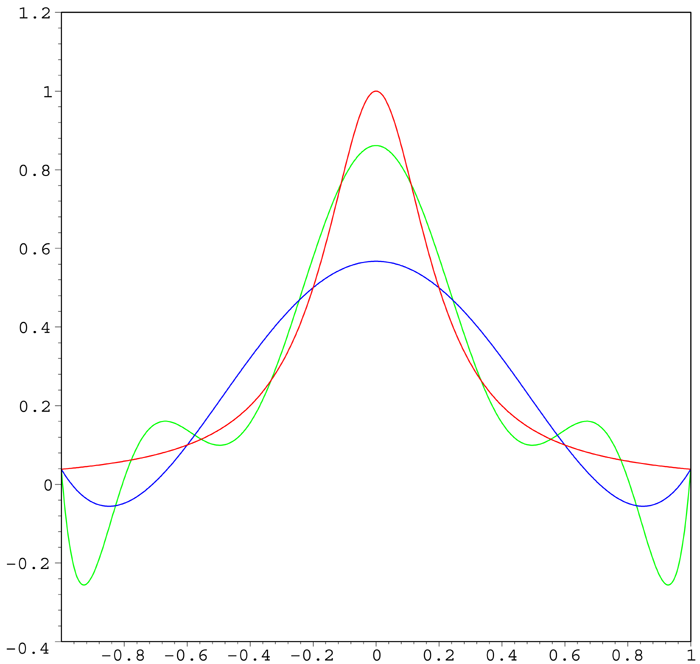
\includegraphics[height=14\baselineskip,
     width=0.5\linewidth]{tema2/Rungesphenomenon}
     \caption{Fenómeno de Runge para $f(x)=1/(1+25x^2)$ (en color
       rojo). En color azul y verde se representan los polinomios de
       interpolación $p_5(x)$ y $p_9(x)$, respectivamente \scriptsize[Fuente:
       \href{http://commons.wikimedia.org}{Wikimedia commons}]}.
     \label{fig:fenomeno-runge}
   \end{figure}
   Si representamos gráficamente el polinomio de interpolación de
   Lagrange, $p_n(x)$ (figura~\ref{fig:fenomeno-runge}), veremos que a
   medida que $n$ crece se producen grandes oscilaciones cerca de los
   extremos del intervalo.
 \end{example}


 La observación anterior es importante, pues significa que \textbf{no siempre
   podemos conseguir mejorar la aproximación de una función mediante el
   incremento del grado del polinomio de interpolación de Lagrange}.
 Obsérvese que este hecho no entra en contradicción con el teorema de
 aproximación de Weierstrass (que afirma que los polinomios son densos
 en las funciones continuas con la norma uniforme). Simplemente: no
 siempre el interpolador de Lagrange es la mejor aproximación por
 polinomios de una función continua.

 Para mitigar este problema existen distintas posibilidades como:
 \begin{enumerate}
 \item Escoger cuidadosamente el soporte de interpolación.
 \item Utilizar interpolación a trozos o funciones \textit{spline}
 \item Renunciar a la interpolación y utilizar otro tipo de técnica
   para la aproximación, como mínimos cuadrados.
 \end{enumerate}

 En la siguiente sección, estudiaremos la segunda de estas
 posibilidades.

 \section{Interpolación a trozos. Funciones \textit{spline} o ranura}
 \label{sec:interp-trozos-splines}

 \subsection{Interpolacion a trozos}
 \label{sec:interpolacion-trozos}


 Dada una función $f$ continua en $[a,b]$, la idea de la interpolación
 a trozos consiste en fijar una partición ${\cal
   P}=\{a=x_0<x_1<\cdots<x_n=b\}$ para aproximar a $f$ mediante
 interpolación de Lagrange en cada uno de los subintervalos
 $[x_{i-1},x_{i}]$, $i=1,...,n$, de modo que el grado de estos
 polinomios, $m$, sea pequeño (en la práctica $m=1$, $2$ ó $3$) y la
 función resultante sea continua entre estos subintervalos.

 Definamos el diámetro de la partición como
 $h=\max_{i\in\{1,...,n\}}(x_i-x_{i-1})$. Nuestro propósito es aumentar
 el número de subintervalos (es decir hacer $n\to \infty$) de forma
 que $h\to 0$, mientras mantenemos constante el grado de los polinomios
 de interpolación.

 Más específicamente, definimos el conjunto de las \resaltar{funciones
   continuas y polinómicas a trozos} como:
 \begin{equation*}
   V_h = \{ q_h\in C^0([a,b]) \ /\ q_h|_{[x_{i-1},x_{i}]}\in \Pol_m[x]\
   \forall i=1,...,n \}.
 \end{equation*}
 Para cada $i=1,...,n$, consideramos el subintervalo $[x_{i-1},x_i]$ y
 definimos $m-1$ nodos interiores, $\xi_{ij}\in (x_{i-1},x_i)$ (con
 $j=1,\dots,m-1$). Para los datos anteriores, definimos la
 \resaltar{función de interpolación polinómica a trozos}, $p_h$, como
 la única función de $V_h$ que en cada intervalo $[x_{i-1},x_i]$
 interpola los valores de $f$ en los $m+1$ nodos situados en $[x_{i-1},
 x_{i}]$.  Es decir, para cada $i=1,\dots n$:
 \begin{align*}
   p_h(x_{i-1})&=f(x_{i-1}),\\
   p_h(\xi_{ij})&=f(\xi_{ij}), \quad j=1,...,m-1,\\
   p_h(x_i)&=f(x_i).
 \end{align*}

 \begin{theorem}[Estimación de error]
   \label{thm:interpol-trozos-error}
   Si $f\in C^{m+1}( [a,b])$ y $p_h$ es el interpolador a trozos
   definido anteriormente:
   \begin{equation}
     ||f-p_h||_\infty\le\frac{M_{m+1}}{(m+1)!}h^{m+1},
     \quad
     \text{ donde } M_{m+1}=||f^{m+1)}||_\infty.
     \label{eq:interpol-trozos-error}
   \end{equation}
 \end{theorem}

 \begin{proof}
   Consideremos $||f-p_h||_{\infty, [a,b]}=\max\{ |f(x)-p_h(x)|\ /\
   x\in[a,b]\}$.
   \begin{itemize}
   \item Este máximo se alcanza en algún subintervalo $[x_{i-1},x_{i}]$
     es decir $||f-p_h||_{\infty}=||f-p_h||_{\infty, [x_{i-1},x_i]}$
     para algún $i=1,\dots,n$.
   \item En este subintervalo podemos usar el
     teorema~\ref{thm:error-interpol-lagrange}, por lo que
     \begin{align*}
       ||f-p_h||_\infty &= ||f-p_h||_{\infty, [x_{i-1},x_i]}  \\
       &\le\frac{M_{m+1}}{(m+1)!}
       (x-x_{i-1})(x-\xi_{i1})\cdots(x-\xi_{i,m-1})(x-x_i).
     \end{align*}
   \end{itemize}
   Como cada uno de estos factores es menor que $h$, finaliza la
   demostración.
 \end{proof}

 \begin{remark}
   \label{rk:3}
   En el caso de interpolación a trozos, podemos garantizar que, si
   $f\in C^{m+1}([a,b])$,
   \begin{equation*}
     ||f-p_h||_\infty \to 0 \quad \text{cuando } h \to 0,
   \end{equation*}
   pues el término $M_{m+1}/(m+1)!$ en~(\ref{eq:interpol-trozos-error})
   depende sólo de $||f^{m+1)}||_\infty$ y $m$, que permanece constante
   a medida que $h\to 0$.
 \end{remark}

 \subsection{Interpolación por funciones \textit{spline} o ranura}
 \label{sec:splines}

 Nos centraremos ahora en
 el caso en que se aumenta la regularidad del interpolante.
 Es decir, dada una partición 
 ${\cal P}= \{a = x_0 <x_1 < \cdots <x_n=b\}$
 del intervalo $[a,b]$ y dados unos datos $y_0$, $y_1$, \dots, $y_n$
 (que eventualmente podrían venir dados como $y_i=f(x_i)$ para alguna
 función $f$), nos proponemos el construir:
 \begin{itemize}
 \item  funciones polinómicas a trozos, en los subintervalos que
   denotaremos $I_i=[x_{i},x_{i+1}]$ (para $ i=0,\dots,n-1$)
 \item que interpolen los valores $\{y_i\}_{i=0}^n$ en el soporte
   $S=\{x_i\}_{i=0}^n$ y
 \item que sean <<regulares>> en $[a,b]$.
 \end{itemize}
 En la práctica, se utiliza regularidad $C^{k-1}([a,b])$, donde
 $k\in\Nset$ es el grado de los polinomios de
 interpolación. Concretamente:% , en lo que sigue nos centraremos en el conjunto:
 % \begin{equation*}
 %   V_h = \{q_h \in C^{k-1}([a,b])\ / \ q_h|_{I_i}}\in
 %   \Pol_k[x],\ \forall i=0,\dots,n-1\},
 % \end{equation*}
 % donde denotamos $I_i=[x_{i+1},x_i]$ para $ i=0,\dots,n-1$.

 \begin{definition}[Funciones spline o ranura]
   \label{def:funcion-spline}
   Sea una partición ${\cal P}= \{a = x_0 <x_1 < \cdots <x_n=b\}$ del
   intervalo $[a,b]$ y unos valores $\{y_i\}_{i=0}^n$. Fijado
   $k\in\Nset$, consideremos el espacio de las funciones que son
   de clase $C^{k-1}$ en $[a,b]$ y que en cada subintervalo son
   polinomios de grado $k$:
   \begin{equation*}
     V_h = \{q_h \in C^{k-1}([a,b])\ / \ q_h|_{I_i}\in  \Pol_k[x],\ \forall i=0,\dots,n-1\}.
   \end{equation*}
   Llamamos función \resaltar{spline} (o \resaltar{ranura}) a
   cualquier $s_h\in V_h$. Decimos que una función spline $s_h\in V_h$
   interpola los datos $\{(x_i,y_i)\}_{i=0}^n$ si $s_h(x_i)=y_i$ para
   todo $i=0,\dots,n$.
 \end{definition}

 Al caso $k=1$ se le llama \textit{spline lineal} y coincide (para
 polinomios de dimensión uno) con la interpolación a trozos estudiada
 en el apartado anterior Al caso $k=2$ se le llama \textit{spline
   cuadrático} y a $k=3$, \textit{spline cúbico}. Splines lineales y
 cúbicos son los más utilizados en la práctica.

 \subsubsection{Splines lineales}
 \label{sec:splines-lineales}

 Consideremos
 \begin{equation*}
   V_h = \{q_h \in C^{0}([a,b])\ / \ q_h|_{I_i}\in  \Pol_1[x],\ \forall i=0,\dots,n-1\}.
 \end{equation*}
 Una función $s_h\in V_h$ que interpole los datos
 $\{(x_i,y_i)\}_{i=0}^n$ queda determinada por las siguientes $n$
 ecuaciones (que resultan de escribir, en cada subintervalo $I_i=[x_i,
 x_{i+1}]$, la ecuación de la recta que pasa por los puntos
 $(x_i,y_i)$ y $(x_{i+1},y_{i+1})$):
 \begin{equation*}
   \label{eq:splines-lineales-1}
   s_h(x) = l_i(x) = y_i + \frac{y_{i+1}-y_i}{x_{i+1}-x_i}(x-x_i) \quad
   \forall x\in I_i.
 \end{equation*}

 \begin{example}
   \label{ex:splines-lineales-1}
   Interpolar, mediante splines lineales, los siguientes
   datos:
   \begin{equation*}
     \{ (1,2),\ (2,-1),\ (3,0),\ (4,1) \},
   \end{equation*}
 \end{example}
 es decir:
 \begin{equation}
   \small
   \begin{array}{r@{\rule{4ex}{0pt}}rrrcr}
     % \toprule
     i & 0 & 1 & 2 & 3 
     \\ \toprule %\cline{1-5}
     x_i & 1 & 2 & 3 & 4
     \\ \midrule
     y_i & 2 & -1 & 0  & 1
     \\
     \bottomrule
   \end{array}
   \label{eq:tabla-datos-lagrange-splines}
 \end{equation}
 Escribiendo las ecuaciones anteriores para los
 estos datos obtenemos:
 \begin{equation*}
   s_h(x)=\left\{
     \begin{tabular}{rll}
       $2 -3 (x-1)$ & si & $x\in[1,2]$,
       \\\noalign{\medskip}
       $-1 + (x-2)$ & si & $x\in[2,3]$,
       \\\noalign{\medskip}
       $0 - (x-3)$ & si & $x\in[3,4]$
     \end{tabular} \right.
   =\left\{
     \begin{tabular}{rll}
       $5 -3x$ & si & $x\in[1,2]$,
       \\\noalign{\smallskip}
       $x-3$ & si & $x\in[2,3]$,
       \\\noalign{\smallskip}
       $x-3$ & si & $x\in[3,4]$.
     \end{tabular} \right.
 \end{equation*}

 \subsubsection{Splines cúbicos}
 \label{sec:splines-lineales}

 Consideremos ahora el espacio
 \begin{equation*} V_h = \{q_h \in C^{2}([a,b])\ / \ q_h|_{I_i}\in
   \Pol_3[x],\ \forall i=0,\dots,n-1\}.
 \end{equation*} Nos proponemos calcular una función $s_h\in V_h$ (un
 spline cúbico) que interpole unos datos determinados,
 $\{(x_i,y_i)\}_{i=0}^n$. Comprobaremos que este problema es
 equivalente a un sistema de ecuaciones lineales.

 En cada intervalo $I_i=[x_i, x_{i+1}]$, el spline cúbico es un
 polinomio de grado tres, es decir, para cada $i=0,\dots,n-1$ se tiene:
 \begin{equation}
   s_h(x) = s_i(x) = a_i + b_ix + c_ix^2 + d_ix^3,\quad
   \forall x\in I_i.
   \label{eq:spline-cubico}
 \end{equation}
 Para calcular el spline $s_h$ es necesario determinar $\{a_i, b_i,
 c_i, d_i\}_{i=0}^{n-1}$, es decir $4n$ incógnitas. Por lo tanto,
 necesitaremos $4n$ ecuaciones, que se obtienen de la siguiente forma:
 \begin{itemize}
 \item $n+1$ condiciones provienen de la interpolación de los datos
   $\{(x_i, y_i)\}_{i=0}^n$:
   $$
   s_i(x_i)=y_i, \quad i=0,1,\dots,n.
   $$
 \item $3(n-1)$ condiciones provienen  de la regularidad de $s_h$ en
   $[a,b]$. En concreto:
   \begin{equation*}
     \left.
       \begin{aligned}
         s_{i-1}(x_i)&=s_{i}(x_i) \quad \text{(continuidad de $s_h$)}
         \\
         s'_{i-1}(x_i)&=s'_{i}(x_i) \quad \text{(continuidad de $s_h'$)}
         \\
         s''_{i-1}(x_i)&=s''_{i}(x_i) \quad \text{(continuidad de $s_h''$)}
       \end{aligned}
     \right\} \quad \forall i=1,\dots,n-1 
   \end{equation*}
 \item Sumando todo, tenemos $(n+1) + 3(n-1) = 4n-2$ ecuaciones, para
   las $4n$ incógnitas de las que partimos. En consecuencia,
   necesitamos $2$ ecuaciones más, que se suelen imponer sobre los
   extremos del intervalo $[a,b]$. Las más utilizadas son:
   \begin{itemize}
   \item Si disponemos de información sobre la derivada en los
     extremos, $y_a'$, $y_b'\in\Rset$, imponemos:
     \begin{equation*}
       s_0'(a)=y_a', \quad s_n'(b)=y_b' \quad \text{(condición de frontera fija)}.
     \end{equation*}
   \item Si carecemos de la información anterior, suele imponerse que
     la segunda derivada se anule en los extremos:
     \begin{equation*}
       s_0''(a)=0, \quad s_n''(b)=0 \quad \text{(condición natural o de
         frontera libre)}.
     \end{equation*}
   \end{itemize}
 \end{itemize}

 \begin{example}
   \label{ex:splines-cubicos}
   A continuación plantearemos el sistema de ecuaciones que resulta al
   usar splines cúbicos naturales para
   interpolar los datos del ejemplo~\ref{ex:splines-lineales-1}. Para
   ello, reescribimos~(\ref{eq:spline-cubico}) como:
   \begin{equation*}
     s_h(x)=\left\{
       \begin{aligned}
         s_0(x)&=a_0 + b_0(x-1) + c_0(x-1)^2 + d_0(x-1)^3 
         & \text{si} && x\in[1,2],
         \\
         s_1(x)&=a_1 + b_1(x-2) + c_1(x-2)^2 + d_1(x-2)^3 
         &\text{si}&& x\in[2,3],
         \\
         s_2(x)&=a_2 + b_2(x-3) + c_2(x-3)^2 + d_2(x-3)^3 
         & \text{si}&& x\in[3,4].
       \end{aligned}\right.
   \end{equation*}
 \end{example}

 Tenemos $12$ incógnitas y disponemos de las siguientes ecuaciones:
 \begin{itemize}
 \item Interpolación:
   \begin{itemize}
   \item Imponiendo $s_h(x_i)=y_i$, $i=0,1,2$, llegamos directamente
     a
     \begin{equation*}
       a_0=2, \quad a_1=-1, \quad a_2=0
     \end{equation*}
   \item Imponiendo $s_h(x_3)=s_2(x_3)=y_3$, llegamos a:
     \begin{equation*}
       a_2+b_2+c_2+d_2=1.
     \end{equation*}
   \end{itemize}
 \item Continuidad:
   \begin{align*}
     s_0(x_1)=s_1(x_1) &\Rightarrow a_0+b_0+c_0+d_0 = a_1,
     \\
     s_1(x_2)=s_2(x_2) &\Rightarrow a_1+b_1+c_1+d_1 = a_2.
   \end{align*}
 \item Continuidad de $s_h'$. Usando que
   $s_i'(x)=b_i+2c_i(x-x_i)+3d_i(x-x_i)^2$:
   \begin{align*}
     s_0'(x_1)=s_1'(x_1) &\Rightarrow b_0+2c_0+3d_0 = b_1,
     \\
     s_1'(x_2)=s_2'(x_2) &\Rightarrow b_1+2c_1+3d_1 = b_2.
   \end{align*}
 \item Continuidad de $s_h''$. Usando que
   $s_i'(x)=2c_i+6d_i(x-x_i)$:
   \begin{align*}
     s_0''(x_1)=s_1''(x_1) &\Rightarrow 2c_0+6d_0 = 2c_1,
     \\
     s_1''(x_2)=s_2''(x_2) &\Rightarrow 2c_1+6d_1 = 2c_2.
   \end{align*}
 \item Además imponemos condiciones naturales en $x_0$ y en $x_3$,
   $s_0''(x_0)=0$, $s_2'(x_3)=0$, de donde:
   \begin{equation*}
     2c_0 = 0, \quad 2c_2 + 6 d_2 =0.
   \end{equation*}
 \end{itemize}

 En notación matricial, tenemos el siguiente sistema de ecuaciones:
 \newcommand{\z}{\color{gray}0}
 \begin{equation*}
   \left[
     \begin{array}{rrrr@{\rule{1.3em}{0pt}}rrrr@{\rule{1.3em}{0pt}}rrrr}
       1&\z&\z&\z& \z&\z&\z&\z& \z&\z&\z&\z \\
       \z&\z&\z&\z& 1&\z&\z&\z& \z&\z&\z&\z \\
       \z&\z&\z&\z& \z&\z&\z&\z& 1&\z&\z&\z \\
       \z&\z&\z&\z& \z&\z&\z&\z& 1&1&1&1 \\\noalign{\medskip}
       
       1&1&1&1& -1&\z&\z&\z& \z&\z&\z&\z \\
       \z&\z&\z&\z& 1&1&1&1& -1&\z&\z&\z \\
       \z&1&2&3& \z&-1&\z&\z& \z&\z&\z&\z \\
       \z&\z&\z&\z& \z&1&2&3& \z&-1&\z&\z \\\noalign{\medskip}

       \z&\z&2&6& \z&\z&-2&\z& \z&\z&\z&\z \\
       \z&\z&\z&\z& \z&\z&2&6& \z&\z&-2&\z \\
       \z&\z&2&\z& \z&\z&\z&\z& \z&\z&\z&\z \\
       \z&\z&\z&\z& \z&\z&\z&\z& \z&\z&2&6 \\
     \end{array}
   \right]
   \
   \left[
     \begin{array}{r}
       a_0 \\ b_0 \\ c_0 \\ d_0 \\ \noalign{\medskip}
       a_1 \\ b_1 \\ c_1 \\ d_1 \\ \noalign{\medskip}
       a_2 \\ b_2 \\ c_2 \\ d_2
     \end{array}
   \right]
   =
   \left[
     \begin{array}{r}
       2 \\ -1 \\ 0 \\ 1 \\ \noalign{\medskip}
       \z \\  \z \\ \z \\ \z \\ \noalign{\medskip}
       \z \\  \z \\ \z \\ \z
     \end{array}
   \right]
 \end{equation*}
 \begin{figure}
   \centering
   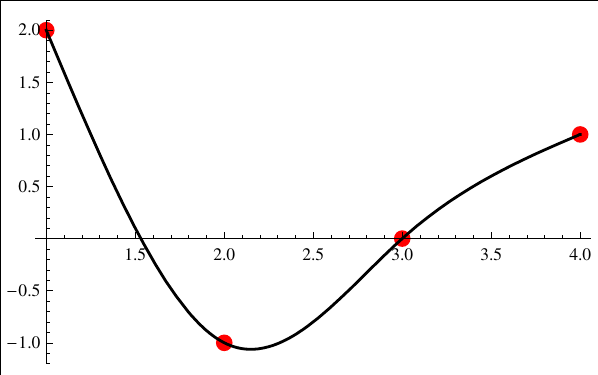
\includegraphics[width=0.4\linewidth]{tema2/spline-cubico}
   \label{fig:spline-cubico} 
   \caption{Spline cúbico que interpola los puntos de la
     tabla~\ref{eq:tabla-datos-lagrange-splines}.}
 \end{figure}
 Se puede demostrar (ver [Burden \& Faires] en la bibliografía) que
 este sistema tiene una única solución y que (como en el caso de
 splines lineales) los splines cúbicos convergen a la función
 interpolada, siempre que ésta sea suficientemente regular. 
 Aunque en el sistema anterior se pueden eliminar fácilmente algunas
 incógnitas ($a_0$, $a_1$, $a_2$ y $c_0$), el sistema resultante
 es de orden $8\times 8$ y en la práctica debe ser resuelto mediante el
 ordenador (especialmente cuando en aumente el número de
 subintervalos). Como resultado, se obtienen los coeficientes de los
 polinomios de grado $3$ en $[1,2]$, $[2,3]$ y $[3,4]$ que definen el
 spline cúbico. Estos polinomios han sido representado en la
 figura~\ref{fig:spline-cubico}.


 % \subsubsection*{En resumen}
 En resumen, en esta sección hemos conseguido mitigar el problema de
 convergencia que puede presenta la interpolación de datos cuando
 aumenta el grado de los polinomios. Para ello se han utilizado de
 funciones polinómicas a trozos y regulares en $[a,b]$, para las que
 hemos probado convergencia uniforme en el caso $C^0([a,b])$. Como
 ejemplo final, se presentan dos imágenes (extraídas de [Burden \&
 Faires]): en la a figura~\ref{fig:pato-alto-orden} se utiliza un
 polinomio de alto orden, generándose grandes oscilaciones. En la
 figura~\ref{fig:pato-spline} se utilizan funciones splines cúbicas,
 obteniéndose excelentes resultados.

 \begin{figure}
   \centering
   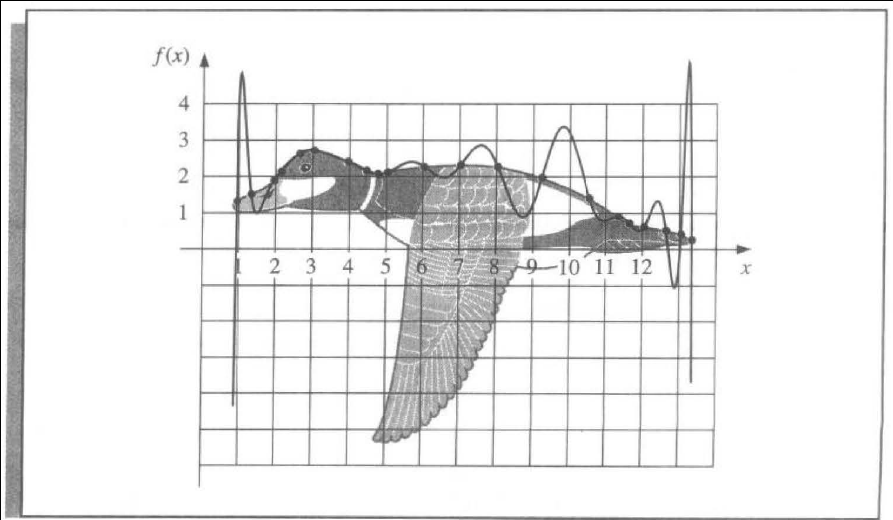
\includegraphics[width=0.75\linewidth]{tema2/pato-interpol}
   \caption{Interpolación con polinomios de alto orden}
   \label{fig:pato-alto-orden}
 \end{figure}

 \begin{figure}
   \centering
   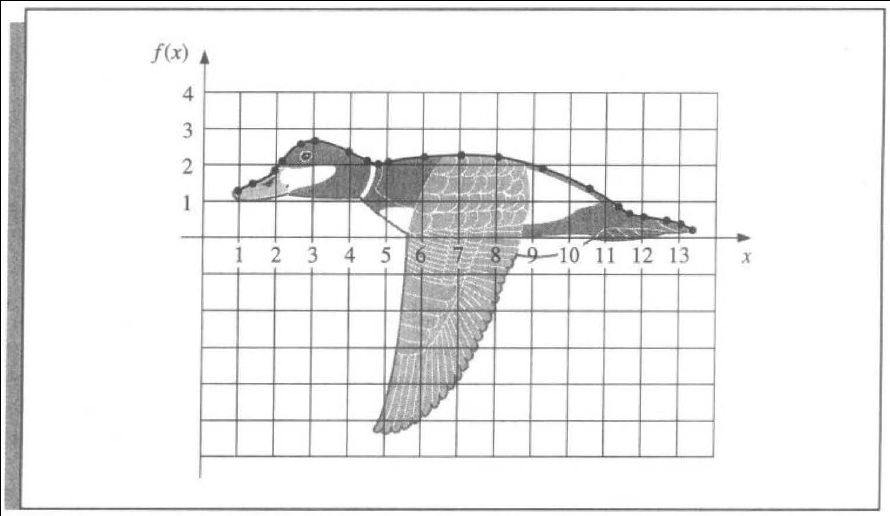
\includegraphics[width=0.75\linewidth]{tema2/pato-spline}
   \caption{Interpolación con splines cúbicos}
   \label{fig:pato-spline}
 \end{figure}


 \section{Interpolación de Hermite}
 \label{sec:interp-de-hermite}

 Consideremos ahora un conjunto de datos definido por un soporte de
 $n+1$ nodos distintos, $S=\{x_0,x_1,\dots,x_n\}\subset \Rset$ junto al
 siguiente conjunto de $2(n+1)$ datos: 
 \begin{equation}
   \{y_0,y_1\dots,y_n\} \cup \{y'_0,y'_1\dots,y'_n\}. 
   \label{eq:datos-hermite}
 \end{equation}
 Con frecuencia, estos datos vienen dados por ciertos valores conocidos
 de una función derivable, es decir  $y_i=f(x_i)$ e
 $y'_i=f'(x_i)$ para alguna función $f$.

 Se trata de encontrar un polinomio $p(x)$ del menor grado posible tal
 que 
 \begin{equation}
   \left.
     \begin{aligned}
       p(x_i) &= y_i \\ p'(x_i)&=y_i'
     \end{aligned}
   \right\}\quad \forall i=0,\dots,n.
   \label{eq:interpolacion-hermite}
 \end{equation}
 Un polinomio con estas características se llama polinomio de
 interpolación de Hermite.

 \subsection{Existencia y unicidad}
 \label{sec:exist-y-unic}

 \begin{theorem}[Existencia y unicidad]
   Dado un soporte de $n+1$ nodos distintos, $x_0$,
   $x_1$,\dots,$x_n\in\Rset$ y dados $2n+2$ datos como
   en~(\ref{eq:datos-hermite}), existe un único polinomio de grado
   $2n+1$ que interpola estos datos, en el sentido
   de~(\ref{eq:interpolacion-hermite}).
 \end{theorem}

 \subsection*{Construcción del polinomio de interpolación de Hermite}
 \label{sec:constr-del-polin-hermite}

 Es posible comprobar que el polinomio de hermite que interpola los
 datos~(\ref{eq:datos-hermite}) en un soporte $\{x_0,\dots,x_n\}$
 viene dado por:
 \begin{equation*}
   p(x)=\sum_{i=0}^{2n+1}(u_i(x)y_i+ v_i(x)y'_i),
 \end{equation*}
 donde
 \begin{align*}
   u_i(x)&=\left[1-2L'_i(x_i)(x-x_i)\right]\, L_i^2(x)
   \\ \noalign{\smallskip}
   v_i(x)&=(x-x_i)\, L_i^2(x),
 \end{align*}
 siendo $\{L_i\}_{i=0}^n$ la base de Lagrange asociada al soporte,
 es decir, cada $L_i$ es el único polinomio de grado $n$ tal que:
 \begin{equation}
   L_i(x_j)= \delta_{ij} = 
   \left\{\begin{array}{l}
       1 \text{ si } i=j, \\\noalign{\medskip} 0 \text{ si } i\neq j
     \end{array}\right.
 \end{equation}

 El inconveniente de esta formulación del polinomio de interpolación de
 Hermite es que es computacionalmente costosa cuando el número de nodos
 es relativamente alto. En la práctica, suele ser más eficiente el
 utilizar la siguiente alternativa, basada en el uso de diferencias
 divididas:


 \begin{theorem}
   \label{thm:formula-newton-hermite}
   Sea $f:[a,b]\to\Rset$ derivable y sea $\{x_i\}_{i=0}^n$ un soporte
   de $n+1$ nodos distintos y ordenados, esto es,
   $x_0<x_1<\cdots<x_n$. Denotemos $z_{2i}=x_i$ y $z_{2i+1}=x_i$, esto es:
   \begin{alignat*}{2} % 2 rl columns
     z_0&=x_0, & z_1&=x_0,\\ 
     z_2&=x_1, & z_3&=x_1,\\ 
     &\ \vdots & &\ \vdots \\
     z_{2n}&=x_n, \qquad & z_{2n+1}&=x_n.
   \end{alignat*}
   Entonces, el polinomio de Hermite puede construirse como:
   \begin{equation*}
     p_{2n+1}(x)=\sum_{i=0}^{2n+1}f[z_0,\dots,z_i]
     (x-z_0)(x-z_1)\cdots(x-z_{i-1}), 
   \end{equation*}
   donde, cuando $z_i=z_{i+1}$, se conviene que $f[z_i,z_{i+1}]=y'_i$.
 \end{theorem}

 \subsection*{Expresión del error}
 \label{sec:expresion-del-error-hermite}

 Para la interpolación de Hermite se tiene una expresión del error
 similar a la obtenida en el teorema~\ref{thm:error-interpol-lagrange}:
 \begin{theorem}
   Sea $f\in C^{2n+2}([a,b])$ y sea $p_{2n+1}(x)$ el polinomio de
   Hermite asociado a los datos $y_i=f(x_i)$, $y'_i=f(x_i)$ para un
   soporte $\{x_i\}_{i=0}^n$. Entonces, para cada $x\in [a,b]$ existe
   $\xi_x\in (a,b)$ tal que:
   \begin{equation*}
     % \label{eq:expresion-error-interpol-hermite}
     f(x)-p_{2n+1}(x)=\frac{f^{2n+2)}(\xi_x)}{(2n+2)!} (x-x_0)^2(x-x_1)^2\dots(x-x_n)^2.
   \end{equation*}
 \end{theorem}

 \section{Aproximación mediante mínimos cuadrados}
 \label{sec:minimos-cuadrados}

 \begin{quotation}
   \it\tiny El día de Año Nuevo de 1801, el astrónomo italiano Giuseppe
   Piazzi descubrió el planeta enano Ceres. Fue capaz de seguir su
   órbita durante 40 días. Durante el curso de ese año, muchos
   científicos intentaron estimar su trayectoria con base en las
   observaciones de Piazzi (resolver las ecuaciones no lineales de
   Kepler de movimiento es muy difícil). La mayoría de las evaluaciones
   fueron inútiles; el único cálculo suficientemente preciso para
   permitir a Franz Xaver von Zach, astrónomo alemán, reencontrar a
   Ceres al final del año fue el de Carl Friedrich Gauss, por entonces
   un joven de 24 años (los fundamentos de su enfoque ya los había
   planteado en 1795, cuando aún tenía 18 años). Sin embargo, su método
   de mínimos cuadrados no se publicó sino hasta 1809, y apareció en el
   segundo volumen de su trabajo sobre mecánica celeste, Theoria Motus
   Corporum Coelestium in sectionibus conicis solem ambientium. El
   francés Adrien-Marie Legendre desarrolló el mismo método de forma
   independiente en 1805.  En 1829, Gauss fue capaz de establecer la
   razón del éxito maravilloso de este procedimiento: simplemente, el
   método de mínimos cuadrados es óptimo en muchos aspectos. El
   argumento concreto se conoce como teorema de Gauss-Márkov.
   \par\hfill
   -- Wikipedia. Último acceso: 7/4/2014.
 \end{quotation}

 Con frecuencia en entornos científicos, la relación entre dos
 variables es solamente conocida como resultados de medidas
 experimentales, de datos estadísticos, etc. Por tanto, los datos están
 sujetos a errores y no tiene sentido el plantear que interpolen
 exactamente una serie de valores. En vez de ello nos planteamos el
 siguiente problema:

 Dados una serie de datos 
 \begin{equation}
   \{(x_0,y_0),(x_1,y_1),\dots,(x_n,y_n)\}, 
   \label{eq:datos-min-cuadrados}
 \end{equation}
 determinar una función, $g(x)$, que sea ``fácil de calcular'' y tal
 que, el error $|y_i-g(x_i)|$ ``sea mínimo'' en un sentido a precisar.

 Este problema se puede generalizar en el siguiente sentido: dado un espacio
 vectorial normado $(V,||\cdot||)$ y dado $U\subset V$, para cada $f\in
 V$ decimos que $\overline u$ es \textit{la mejor aproximación} a $f$
 en $U$ si se verifica:
 \begin{equation*}
   ||f-\overline u|| \le ||f-u||, \quad \forall u\in U.
 \end{equation*}
 Por falta de espacio, no abordaremos el estudio del problema de la
 mejor aproximación y nos centraremos en el caso de la 
 aproximación mediante mínimos cuadrados lineales.

 En concreto, dados los datos~(\ref{eq:datos-min-cuadrados}), nos
 proponemos hallar una función afín (una recta)
 \begin{equation}
   g(x)=ax+b, \quad a,b\in\Rset,\label{eq:5}
 \end{equation}
 tal que
 \begin{equation*}
   m(a,b) := \sum_{i=0}^n
   \left(
     y_i - g(x_i)
   \right)^2
   =
   \left(
     y_i - a x_i - b
   \right)^2
 \end{equation*}
 sea mínimo (figura~\ref{fig:min-cuadrados-lineales}).

 \begin{figure}
   \centering
   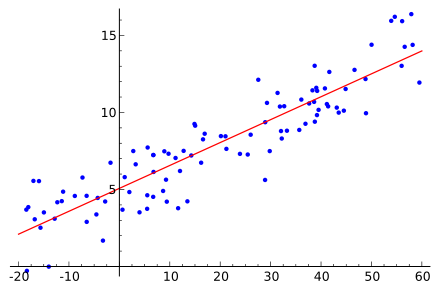
\includegraphics[width=0.6\linewidth]{tema2/linear_regression}
   \caption{Mínimos cuadrados lineales}
   \label{fig:min-cuadrados-lineales}
 \end{figure}

 Para ello:
 \begin{align*}
   \frac{\partial m}{\partial a} & = 
   -2\sum_{i=0}^n
   x_i\left(
     y_i - a x_i - b
   \right) = 
   -2\sum_{i=0}^n x_i y_i
   +2a\sum_{i=0}^n x_i^2
   +2b\sum_{i=0}^n x_i
   = 0
   \quad \text{y} \\
   \frac{\partial m}{\partial b} & = 
   -2\sum_{i=0}^n
   \left(
     y_i - a x_i - b
   \right) = 
   -2\sum_{i=0}^n  y_i
   +2a\sum_{i=0}^n x_i
   +2nb
   = 0.
 \end{align*}

 Basta resolver este sistema lineal de ecuaciones con incógnitas $a$ y
 $b$ para obtener la recta~(\ref{eq:5}) que buscamos:
 \begin{center}
   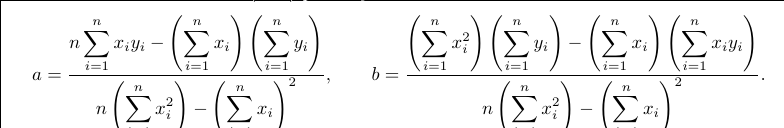
\includegraphics[width=0.9\linewidth]{tema2/ecuacion-min-cuadr}
 \end{center}

 La idea anterior es generalizable a otro tipo de funciones, $g(x)$,
 por ejemplo funciones cuadráticas (aproximación mediante polinomios de
 grado dos).  En prácticas de ordenador veremos algunos ejemplos de
 aproximación mediante mínimos cuadrados.

 %%% Local Variables:
 %%% mode: latex
 %%% TeX-master: "../apuntes-MNII.tex"
 %%% End: 
